%
%     hw6_bbordwell.tex
%     Baylee Bordwell (baylee.bordwell@colorado.edu)
%     Based on the template by Benjamin Brown (bpbrown@colorado.edu)
%     Aug 27, 2014
%
%     Problem set 6 for ASTR/ATOC 5540, Mathematical Methods, taught at
%     University of Colorado, Boulder, Fall 2014.
%
%

\documentclass[10pt, preprint]{aastex}
% formatting based on 2014 NASA ATP proposal with Jeff Oishi

%%%%%%begin preamble
\usepackage[hmargin=1in, vmargin=1in]{geometry} % Margins
\usepackage{hyperref}
\usepackage{url}
\usepackage{times}
\usepackage{natbib}
\usepackage{graphicx}
\usepackage{amsmath}
\usepackage{amsfonts}
\usepackage{amssymb}
\usepackage{pdfpages}
\usepackage{import}
% for code import
\usepackage{listings}
\usepackage{color}
\usepackage{ragged2e}

\hypersetup{
     colorlinks   = true,
     citecolor     = gray,
     urlcolor       = blue
}

%% headers
\usepackage{fancyhdr}
\pagestyle{fancy}
\lhead{ASTR/ATOC 5540}
\chead{}
\rhead{name: Baylee Bordwell}
\lfoot{Problem Set 6}
\cfoot{\thepage}
\rfoot{Fall 2014}
% no hline under header
\renewcommand{\headrulewidth}{0pt}

\newcommand{\sol}{\ensuremath{\odot}}

% make lists compact
\usepackage{enumitem}
%\setlist{nosep}

%%%%%%end preamble


\begin{document}
\section*{Problem Set 6: Detrending Kepler Data, part III}
\begin{enumerate}
\item Based on the fact that it was taking over an hour to not even begin to converge for the Gauss-Seidel method that I used throughout this assignment (so it does work), I only have values for the SOR method with a pre-conditioned matrix.

\begin{table}[!ht]
\centering
\begin{tabular}{l c c c c}
  \bf{Method} & \bf{N = 2 Solution} & \bf{Time (s)} & \bf{Steps} & \bf{Tol.}\\ \hline
  Normal eq. & $y=$(2.52985e+05)$+x$(-2.29530e+02)$+x^2$(2.88217e-01) & 5.064e-4 & 3 & N/A \\
  QR & $y=$(2.52985e+05)$+x$(-2.29530e+02)$+x^2$(2.88217e-01) & 1.543e-4 & 3 & N/A \\
  SOR &  $y=$(2.52998e+05)$+x$(-2.29619e+02)$+x^2$(2.88365e-01) & 49.642 & 105760 & 1e-8\\
\end{tabular}
\end{table}
The behavior of the direct solvers for the first 10 polynomials is described in Figure \ref{fig1}.
\begin{figure}[!ht]
  \centering
  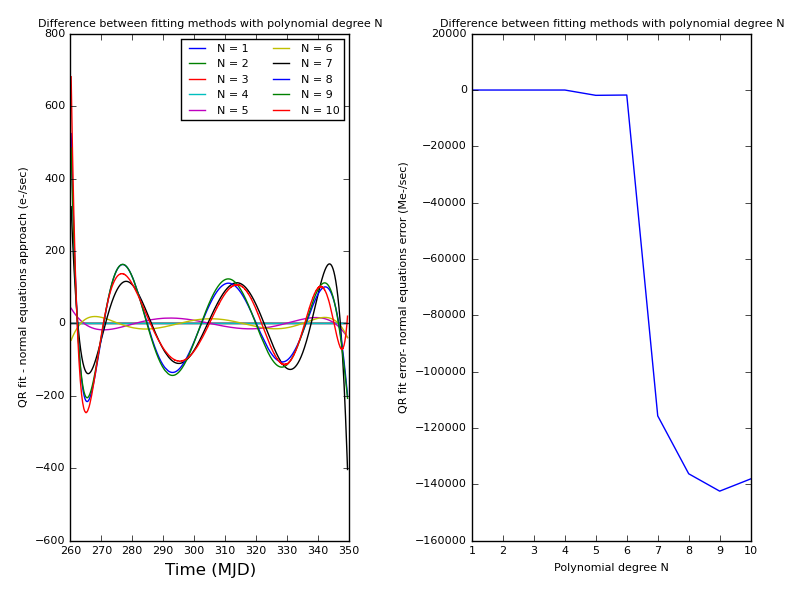
\includegraphics[width=4in]{hw6_fig1_unc.png}
  \caption{\centering Behavior of direct solvers on unconditioned data. \label{fig1}}
\end{figure}


\item Preconditioning the data matrix led to a rapid decrease in the number of steps and required to achieve a high-fidelity solution. The difference was about 3 orders of magnitude for the SOR method. The condition number $\kappa(A)$ went from 1.460e7 to 23.02 with preconditioning and $\kappa(A^TA)$ went from 2.133e15 to 513.

\begin{table}[!ht]
\centering
\begin{tabular}{l c c c c}
  \bf{Method} & \bf{N = 2 Solution} & \bf{Time (s)} & \bf{Steps} & \bf{Tol.}\\ \hline
  Normal eq. & $y=$(2.12770e+05)$+x$(-7.09679e+03)$+x^2$(2.29583e+03) & 5.064e-4 & 3 & N/A \\
  QR & $y=$(2.12770e+05)$+x$(-7.09679e+03)$+x^2$(2.29583e+03) & 1.543e-4 & 3 & N/A \\
  Gauss-Seidel &  $y=$(2.12771e+05)$+x$(-7.09736e+03)$+x^2$(2.29639e+03) & 5.03e-2 & 1032 & 1e-8\\
  SOR &  $y=$(2.12771e+05)$+x$(-7.09475e+03)$+x^2$(2.29391e+03) & 3.55e-2 & 527 & 1e-8\\
\end{tabular}
\end{table}
The behavior of the direct solvers for the first 10 polynomials on the preconditioned data is described in Figure \ref{fig2}.
\clearpage
\begin{figure}[!ht]
  \centering
  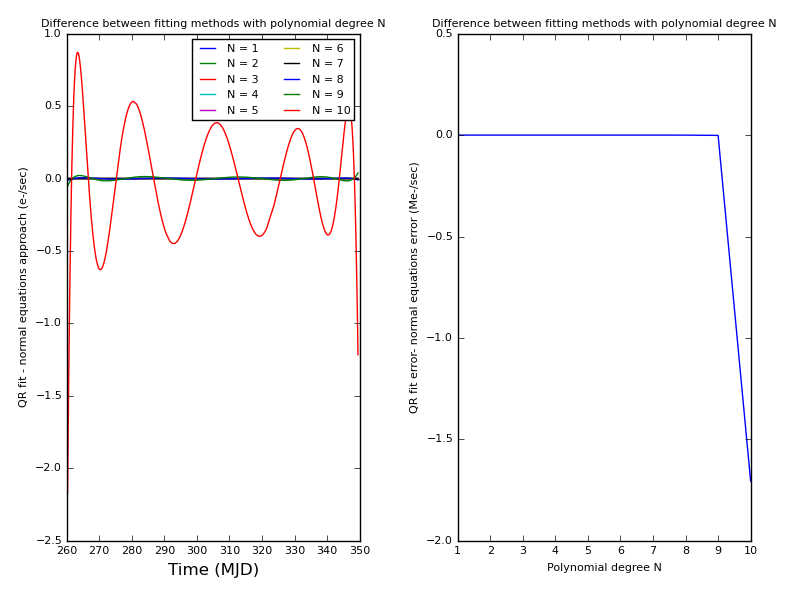
\includegraphics[width=4in]{hw6_fig1a.png}
  \caption{\centering Behavior of direct solvers on preconditioned data. \label{fig2}}
\end{figure}



\item The convergence of both of these methods is described in Figure \ref{fig3}. Adding another degree to the polynomial caused a 20x slow down for the Gauss-Seidel method and 5x slow down for SOR. The effect on the direct solvers was approximately null.
\begin{table}[!ht]
\centering
\begin{tabular}{l c c c c}
  \bf{Method} & \bf{N = 3 Solution} & \bf{Time (s)} & \bf{Steps} & \bf{Tol.}\\ \hline
  Normal eq. & $y=$(2.12425e+05)$+x$(-2.87546e+03)$+x^2$(-8.31596e+03 )$+x^3$(7.08335e+03) 
  & 5.748e-4 & 4 & N/A \\
  QR         & $y=$(2.12425e+05)$+x$(-2.87546e+03)$+x^2$(-8.31596e+03 )$+x^3$(7.08335e+03) 
  & 1.802e-4 & 4 & N/A \\
  Gauss-Seidel & $y=$(2.12426e+05)$+x$(-2.87626e+03)$+x^2$(-8.31399e+03 )$+x^3$(7.08206e+03) 
  & 1.468 & 18763 & 1e-9 \\
  SOR &  $y=$(2.12426e+05)$+x$(-2.87669e+03)$+x^2$(-8.31350e+03 )$+x^3$(7.08197e+03) 
  & 0.1842 & 3494 & 1e-8 \\
\end{tabular}
\end{table}


\item Figure \ref{fig3} shows the convergence of all 4 iterative methods. Conjugate is the fastest by far, and steepest descent is almost 20x slower than the Gauss-Seidel method.

\begin{table}[!ht]
\centering
\begin{tabular}{l c c c c}
  \bf{Method} & \bf{N = 3 Solution} & \bf{Time (s)} & \bf{Steps} & \bf{Tol.}\\ \hline
  Normal eq. & $y=$(2.12425e+05)$+x$(-2.87546e+03)$+x^2$(-8.31596e+03 )$+x^3$(7.08335e+03) 
  & 5.748e-4 & 4 & N/A \\
  QR         & $y=$(2.12425e+05)$+x$(-2.87546e+03)$+x^2$(-8.31596e+03 )$+x^3$(7.08335e+03) 
  & 1.802e-4 & 4 & N/A \\
  Gauss-Seidel & $y=$(2.12426e+05)$+x$(-2.87626e+03)$+x^2$(-8.31399e+03 )$+x^3$(7.08206e+03) 
  & 1.468 & 18763 & 1e-9 \\
  SOR &  $y=$(2.12426e+05)$+x$(-2.87669e+03)$+x^2$(-8.31350e+03 )$+x^3$(7.08197e+03) 
  & 0.1842 & 3494 & 1e-8 \\
  Conjugate gradient &  $y=$(2.12423e+05)$+x$(-2.87389e+03)$+x^2$(-8.31392e+03 )$+x^3$(7.08535e+03) 
  & 6.71e-4 & 15 & 1e-4 \\
  Steepest descent &  $y=$(2.12426e+05)$+x$(-2.87625e+03)$+x^2$(-8.31304e+03 )$+x^3$(7.08210e+03) 
  & 20.958 & 55256 & 1e-9 \\
\end{tabular}
\end{table}

\begin{figure}[!ht]
  \centering
  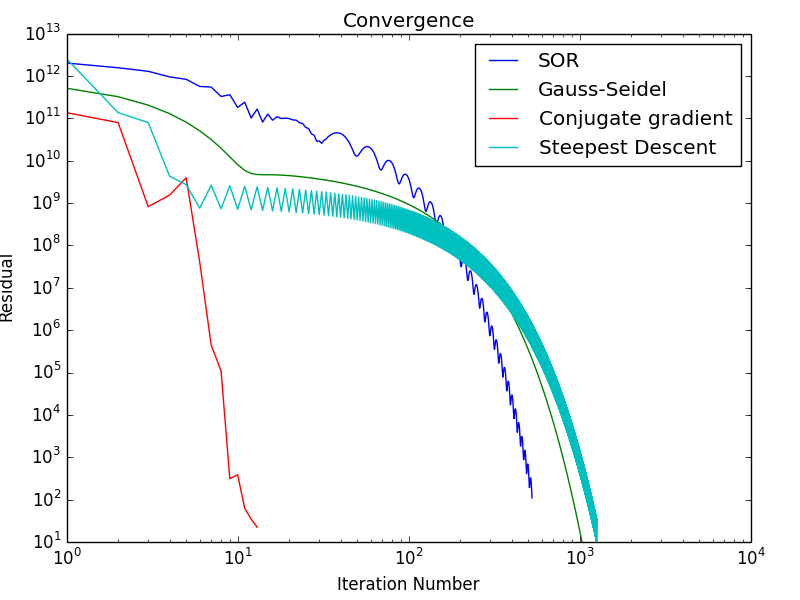
\includegraphics[width=4in]{hw6_fig3.png}
  \caption{\centering Convergence of our iterative methods for N=3 \label{fig3}}
\end{figure}


\item Iterative methods vary from being very fast to very slow. While it would always be preferable, based solely on the data we have here, to use a direct solve, the conjugate gradient comes very close to being on the same timescale as direct solves, and therefore would be ideal for problems that must be solved iteratively.

\end{enumerate}

Code used in this assignment can be found at \url{https://github.com/brbordwell/ASTR_5540/HW6}
\end{document}
